\section{Second industrial benchmark}

\begin{table} %[tbp]
%\begin{wraptable}[10]{r}{9cm}
\centering
\begin{tabular}{l| c c c c c}
& $n_{Literals}$ & $n_{Clauses}$ & $n_{test}$ & $avg(n_{bb})$ &  Filesize \\
\hline
$POF_1$ & 469 & 66957 & 407 & 355.24 & 817 KiB \\
$POF_2$ & 5055 & 81267 & 948 & 1841.5 & 1401 KiB \\
\end{tabular}
\caption[Size comparison of the two $POF$ formulae. ]{Size comparison of the two $POF$s. 
%$n_{test}$ denotes the number of tests executed on the formula.
$n_{test}$ denotes the number of backbone sets to be computed for the formula. $avg(n_{bb})$ is the size of the backbones averaged over all tests.
}
\label{tab:indusComp}
%\end{wraptable}
\end{table}

In the following I will analyze another product formula $POF_2$, similar to the one in the previous chapter. This one, however, is much larger than the previous one, see table \ref{tab:indusComp}. I tested this formula against the same set of algorithms as the previous formula $POF_1$ including $PB3$, to identify the specific characteristics of it and identify the optimal backbone solver for it, just as in the previous section. Table \ref{tab:vonThore2pof} shows the performance results\footnote{Again, the duration of the last SAT call is missing, because it generally took less than a millisecond and could not be measured properly.}.


\begin{wraptable}{R}{7.5cm}
\begin{tabular}{l| c c c}
& $t_{calc}$ & $t_{sat}$ & $n_{sat}$ \\
 \hline
$BB$ 				& 964.05 & 680.113 & 2,063,982\\
$BB_{unit}$ 		& 1229.866 & 429.248 & 417,846\\
$IBB$ 				& 1244.075 & 832.699 & 432,408\\
$PB0$ 				& 427.187 & 276.132 &  129,943\\
$PB0_{model}$ 		& 304.072 & 273.185 &  130,099\\
$PB1$ 				& 498.542 & 316.225 & 146,349\\
$PB1_{model}$ 		& 375.146 & 325.547 &  151,119\\
$PB1_{rotate}$ 		& 614.978 & 311.232 &  141,126\\
$PB1_{forget}$ 		& 471.434 & 292.868 &  143,406\\
$PB1b$ 				& 1333.112 & 818.313 &  460,292\\
$PB1c$ 				& 508.382 & 318.489 &  146,799\\
$PB1c_{5\%}$ 		& 575.371 & 355.767 &  198,242\\
$PB1c_{0.5\%}$ 		& 805.314 & 511.091 &  273,882\\
$PB1d_{50\%}$ 		& 517.259 & 317.346 & 146,430\\
$PB1e$ 				& 509.053 & 314.43 &  148,096\\
$PB2$ 				& 1515.258 & 1025.452 &  437,898\\
$PB2_{5\%}$ 		& 1459.938 & 969.117 &  439,641\\
$PB3$ 				& 363.885 & 318.21 &  146,498\\
\end{tabular}
\caption[Performance results of second industrial benchmark]{Second Industrial benchmark. Values are not averaged, but summed up over 948 different backbone computations.}
\label{tab:vonThore2pof} %for referencing
\end{wraptable}

The first thing that shows, again, is that algorithms with preferences have a much better performance overall. $PB0$ and $PB1$ finish between two and three times faster than $BB$ and $IBB$. Something similar can be seen when you compare $PB1b$ with the $PB2$ variants, however it becomes more complicated to explain the result of $PB1_{forget}$, which outperformed $PB1$ slightly. Perhaps $POF_2$ contains easy components as well as difficult ones. If so, forgetting preferences could adjust to both dynamically during the same model computation, by only dropping preferences about complicated variables. This would be supported by the fact that $PB1_{forget}$ turned out to be the fastest of the $PB1$ variants when it comes to pure SAT time.

Additionally, it seems that model reduction does not give a real benefit in this instance. $PB1_{model}$ outperforms the base configuration with prime implicant reduction as well as $PB1_{rotate}$ and the same goes for the comparison between $PB0$ and $PB0_{model}$. Looking for required literals in the model\footnote{I.e. employing $PB1_{rotate}$} does give a performance benefit visible in the number of SAT calls and the pure calculation time, as is to be expected from the strongest model reduction scheme. It is however negligible. A more interesting case is $PB3$. Here the overall computation time is comparatively close to the pure SAT time, which coincides with the fact that $PB3$ reduces its model only once. However, $PB3$ is still outperformed by $PB0_{model}$. I also tried out the combination of forgetting preferences and not employing model reduction, but their benefits did not add up to result in a better method than $PB0_{model}$. This was done based on the $PB1$ algorithm, because the preferences scheme cannot be modified in $PB0$.

Further we can see that the observation about unit implied backbone literals can be observed again in this benchmark. The number of SAT calls and the time spent in the SAT solver are much better in $BB_{unit}$ compared to $BB$. But this does not reflect in better overall performance. Also, learnable literals don't seem to be particular valuable in this formula as can be deducted from the results of $PB1e$.

Judging from this, the best backbone computation strategy for $POF_2$ would be the $PB0$ algorithm without any model reduction.





%\newpage






\subsection{Efficiency over all assumptions}
In both $POF$ benchmarks, the same formula is worked on hundreds of times. Therefore, it makes sense to think about ways how to make this outer loop efficient as well.


\subsubsection{Resetting formula object}
The first consideration should be to reuse the formula object. The first time that I ran the 407 backbone computations for $POF_1$ with the algorithm $PB3$, the backbone computations by themselves took a sum of 1.5 seconds, but the loop overall took 3.9 seconds. The difference consisted of primarily the copying of the formula(2.2 seconds) and writing down benchmark information(around 150 milliseconds). Lacking deeper understanding of the $Sat4J$ library, at that time I created a new formula object\footnote{The class name in $Sat4J$ is $Solver$ or $ISolver$.} for each backbone computation and copied over the clauses from an unsolved formula object. But it would be much faster to just reuse the same one.

To do this in $Sat4J$ you can reset it. In the case of model enumeration algorithms like $IBB$\footnote{
	Note that the implementations of $BB$ and $IBB$ supplied by $Sat4J$ are already properly configured in a way that formula objects can immediately be reused.
} or $PB1$, this incorporates removing all the blocking clauses because they modify the formula. If you don't do this, all backbone computations after the first one will immediately fail, because the final blocking clause makes the formula unsatisfiable. Additionally, you must flush the set of learned clauses and literals because some of these may be based on the blocking clauses. Therefore, if you would leave them in place, they could reproduce some of the effects that the blocking clause had. Take care that all of this happens in a way that during the individual backbone computations, the learned clauses stay in place. $Sat4J$ supplies a special function to remove a clause under the expectation that it will immediately become subsumed or already is, which you can use to remove old blocking clauses during the loop without flushing the learned clauses. Alternatively you could remove all of them at the end. The ordinary function to remove a clause in $Sat4J$ triggers the cleanup automatically. 

Additionally, it makes sense to revert the decision heuristic if you replaced it with something that allows to implement preferences and you want to reuse the formula object with a backbone solver without them. The typical behaviour throughout the $Sat4J$ library, including the $BB$ and $IBB$ backbone solvers, is to assume that such a data structure is already set up correctly.

One last bit of state inside the formula object that I noticed were two floating point numbers called $claInc$ and $claDecay$. These influence the scale in which the activity values inside the decision heuristic grow and shrink. They do not influence the calculation result, but merely the exact behaviour of the solver.

With all of this taken care of, the duration of the outermost loop over the assumptions took just as long as the sum of the durations of the backbone computations.


\subsubsection{Prepared formulae}
\begin{wraptable}[20]{R}{8cm}
\begin{tabular}{l | c c c}
$Computation$ & $t_{full}$ & $t_{sat}$ & $n_{sat}$\\
\hline 
BB 			& 980.539 & 672.579 & 2,080,370 \\
IBB 		& 1227.487 & 776.105 &  461,746 \\
PB0 		& 374.425 & 219.909 &  129,912 \\
PB0(model) 	& 250.473 & 219.202 &  129,912 \\
PB1 		& 412.914 & 238.005 &  137,985 \\
PB1(model) 	& 290.615 & 244.659 & 140,790 \\

%PB3 & 2093.709 & 1941.915 & 3.343 & 284062\\
\hline \hline 
$Preparation$ & $t_{calc}$ & $n_{learned}$ & $n_{BB}$  \\
\hline
BB         & 1.928 & 1898 & 1,449 \\
PB0        & 0.918 & 2214 & " \\
PB0(model) & 0.505 & 2244 & " \\

\end{tabular}
\caption[Performance results with a prepared formula object]{Benchmark results with reuse of learned clauses and backbones of the base formula $POF_2$. Subsequently number of learned clauses and backbone literals through preparation.}
\label{tab:pofPrepBenefit}
\end{wraptable}
Another good strategy would be to first compute information of the base formula $POF$ and reuse it in all subsequent computations, where the backbone under an assumption was calculated. Two interesting pieces of this would be the clauses that would be learned by doing this and secondly the backbone of the base formula. Both of these are valid for any $POF \cup \{a\}$ because, when a clause gets added to a CNF formula, its set of models can only shrink, no new model can be induced through an additional clause\footnote{Assuming that no new variable was introduced.}. This implies that an assignment that didn't occur in the models before will also not appear in the new smaller set of models, in turn implying that if a variable always occured with the same assignment in $POF$, it will also do so in $POF \cup \{a\}$.


The gain of this depends on the formula. $POF_1$ by itself actually had neither backbone literals %\footnote{	This actually makes a lot of sense. The backbone of a formula consists of all assignments that have to be done to end up in a model. In the context of a product formula, which we have here, this would mean, that a specific feature of the product would always have to be selected. In other words, the product has an option that is not optional.}
nor was it necessary for the SAT solver to learn any new clauses to find a model for it, and even when I tried to compute its backbone with either $PB0$ or $BB$\footnote{Both algorithms, that can leave their learned clauses in place after backbone computation.} in an effort to learn as much about the formula as possible, not a single clause was learned.

$POF_2$ on the other hand actually had quite a large backbone and many clauses to learn. The $Computation$ section of table \ref{tab:pofPrepBenefit} shows performance results where the base formula was always copied from a formula object that was already solved with the $PB0$ algorithm employing prime implicant reduction. With this method, the formula had learned 2214 clauses that its copies would treat as a clause that was explicitely written in the original formula $POF_2$. The $Preparation$ section shows how long the backbone computation of the base formula took with different solvers and how many clauses were learned and additionally the size of $POF_2$'s backbone.

In comparison with unprepared computations (see table \ref{tab:vonThore2pof}), the algorithms that benefitted from this approach were those that employed preferences being all around 20\% faster with a prepared formula object. On the other hand, the $IBB$ algorithm doesn't seem to be affected much and the $BB$ algorithm was even slightly hindered by it. It seems that for this particular benchmark the primary benefit of using a prepared formula lies in that it counters the negative sideeffects of preferences.




\subsubsection{Reusing formula instance}
But why should you discard any information about the formula at all? Both $BB$ and $PB0$ never change their formula during the whole benchmark, so you would think that all of these learned clauses would be just as valuable in subsequent iterations of this benchmark. When you have an object representing a formula in $Sat4J$, calculate its backbone with either $PB0$ or $BB$ and put that into an infinite loop, the duration of each repetition will quickly decrease to only a handful of milliseconds, because all possible conflicts will eventually be evaded with help of knowledge from previous repetitions.

\begin{table}[h]
%\begin{wraptable}{l}{7.5cm}
\centering
\begin{tabular}{l| c c  c}
& $t_{calc}$ & $t_{sat}$ &  $n_{sat}$ \\
\hline
$BB$ & 1275.055 & 829.091 &  2,116,264 \\
%$IBB$ & 1312.134 & 878.177  & 431,554 \\
$PB0$ & 487.614 & 287.116 &  129,626 \\
$PB0_{model}$ & 316.511 & 285.347 & 129,668 \\
\end{tabular}
\caption{Results with a reused formula object and assumptions instead of formula modifications.}
\label{tab:pofAssump}
%\end{wraptable}
\end{table}

However, taking a look at table \ref{tab:pofAssump}, this is clearly not happening. $BB$, $PB0$ and $PB0_{model}$ are 32\% , 14\% and 4\% slower respectively than when using a fresh or resetted formula object without any learned clauses\footnote{For which results are listed in table \ref{tab:vonThore2pof}}. Results for the previous benchmark $POF_1$ were inconclusive with negligible performance differences.

Appearantly, the $POF$ formulae don't benefit much from this technique. It could be that they contain clause clusters that only become problematic with the right variable being fixed to a certain value. In this case the clauses learned during the computation of a backbone under one assumption would be much less useful for the backbone under another assumption. 

Note also that in the domain of SAT solving it is generally considered a bad thing to have many clauses in your formula that aren't useful to the current computation. Even if they are effectively meaningless in the context of their own formula, they have to be checked whether they indicate a unit assignment every time that a relevant variable is assigned a value. Typically a SAT solver removes unused learned clauses regularly, however in this benchmark, this never happened, even over 948 backbone computations, finally having learned 35,983 clauses but not having become noticeably faster.

In fact, as figure \ref{fig:reusePrep} shows, it became slower. Here, the grey continuous line shows the overall computation duration of the $PB0_{model}$ algorithm with reusing the same formula object, while the dashed black line denotes the computation time of the same algorithm solving a prepared formula object and discarding all newer learned clauses. The latter is is faster in every single case, while the grey line even increases its performance loss through its build-up of learned clauses. 


\begin{figure}[h]
\centering
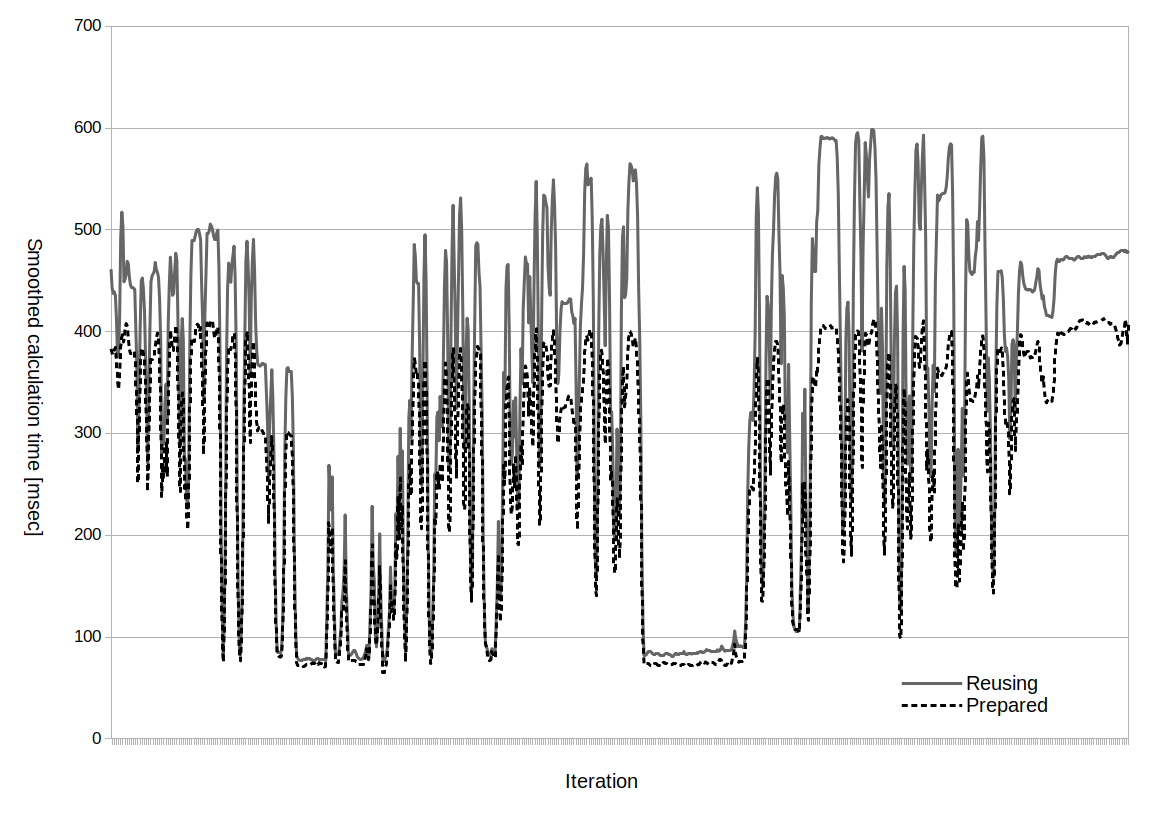
\includegraphics[angle=90,origin=c,width=\textwidth,height=\textheight,keepaspectratio=true]{reuseprep}
\caption[Performance comparison of using a prepared formula object and reusing the same one.]{Performance comparison of using a prepared formula object (dashed black) and reusing the same one (grey) with algorithm $PB0_{model}$. Values are smoothed over a five element window with weights $[\frac{1}{10},\frac{1}{5},\frac{2}{5},\frac{1}{5},\frac{1}{10}]$.}
\label{fig:reusePrep}
%\end{wrapfigure}
\end{figure}

%\newpage
%TODO vergleichs bild zwischen $PB0_model(prepped)$ und $PB0_model(chained)$, am besten geglättet


\iffalse



wenn man BB oder PB0 in einer schleife auf dieselbe formel laufen lässt, geht computation time gegen 0, weil alles gelernte wieder verwendet wird. Ist nicht so.

muss auch berücksichtigen, dass mehr klauseln mehr overhead durch propagation bedeuten
There is however the possibility, that after one backbone computation, the formula object would contain information, that could be valuable to another backbone computation.

TODO: mit vonThore ausprobieren, vielleicht gibts da mehr zu lernen nein gibts nicht, nicht jenseits der grenze zum rauschen.





%%%%%%%%%%%%%%%%%%%%%%%%%%%%%%%%%%%%%%%%%%%%%%%%%%%%%%%%%%%%%%%%%%%%%%%%%%%%%%%%%%%%

%eigentlich erstes: kopieren rausoptimieren


learned lits übernehmen in POF ist schlechter ansatz, weil wird relativ schnell schlechter als immer die formel übernehmen, womöglich nutzlose learned clauses, die nur verlangsamen und nichts aussagen (weil von anderen assumptions)


%%%%%%%%%%%%%%%%%%%%%%%%%%%%%%%%%%%%%%%

The first consideration was to first compute information of the base formula and reuse it in all subsequent computations, where the backbone under an assumption was calculated. However this was not possible.\\
One interesting piece of information would have been the set of clauses that were learned during the computation of a model of the base formula $POF_1$. However this set was empty. Appearantly the formula is simple enough, that the model can be found without a single conflict. The solver returned without having learned any new clause for the formula.

Another thing I thought about was the backbone of the base formula. If you can determine backbone literals of $POF_1$, then you can safely assume, that all of these are part of any restricted formula $POF_1 \cup \{a\}$. This is because, when a clause gets added to a CNF formula, its set of models can only shrink, no new model can be induced through an additional clause\footnote{Assuming that no new variable was introduced.}. This implies that an assignment that didn't occur in the models before will also not appear in the new smaller set of models, in turn implying that if a variable always occured with the same assignment in $POF_1$, it will also do so in $POF_1 \cup \{a\}$. \\
However this set was empty as well and for a good reason in this particular case. The backbone of a formula consists of all assignments that have to be done to end up in a model. In the context of a product formula, which we have here, this would mean, that a specific feature of the product would always have to be selected. In other words, the product has an option that is not optional. 

\fi